\chapter{The LHC and the CMS Experiment}
\section{The Large Hadron Collider}

The state-of-the-art experiments in the field of high energy physics are at the European Organization for Nuclear Research (CERN), where the Large Hadron Collider (LHC) and its complex of accelerators is hosted (Fig. \ref{cernplot}).
\begin{figure}[htb!!!!]
\centering
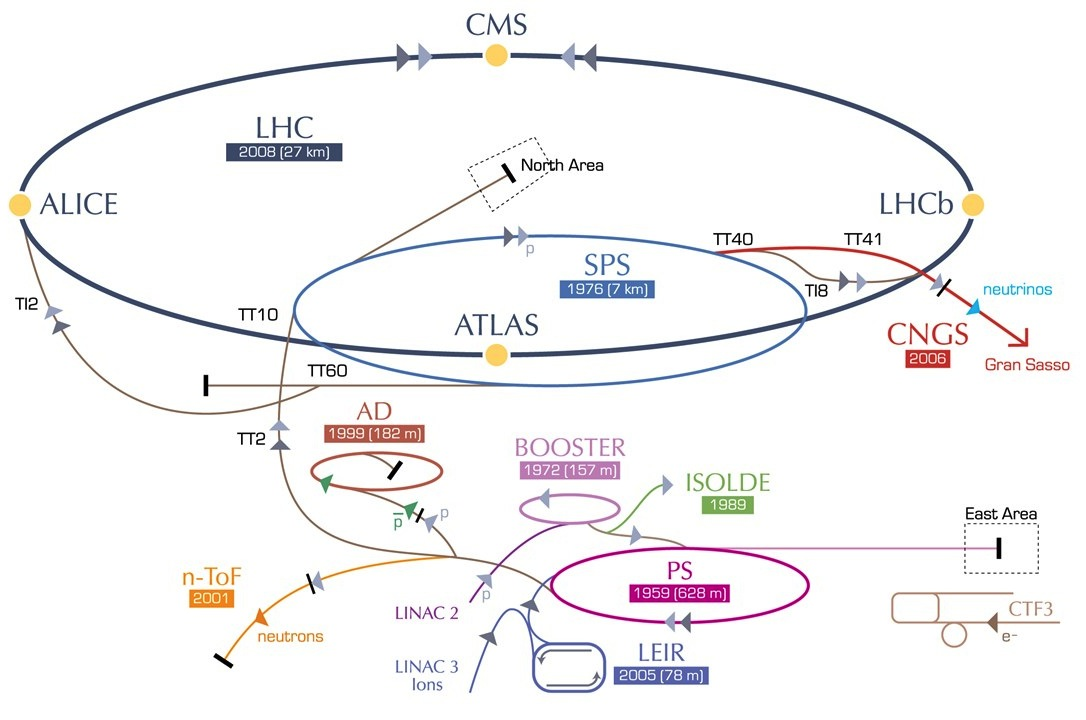
\includegraphics[scale=0.65]{figures/experiment/cernComplex.jpg}
\caption[CERN's Accelerator Complex]{Overview of the CERN's accelerator complex \cite{Mobs:2225847}.}
\label{cernplot}
\end{figure}

The LHC is a circular accelerator with 27 km of circumference installed in a tunnel 50 to 175 meters underground. It was originally designed to collide protons at a centre-of-mass energy of 14 TeV with a design luminosity of $10^{34}$ cm$^{-2}$s$^{-1}$, with the possibility of colliding also heavy ions in different configurations. 

In a circular accelerator such as the LHC, radio-frequency cavities provide the boost while dipole superconducting magnets (Fig. \ref{dipole}) supply the bending magnetic field that keeps the protons in orbit.

\begin{figure}[h!!!!]
\hspace{-0.5cm}
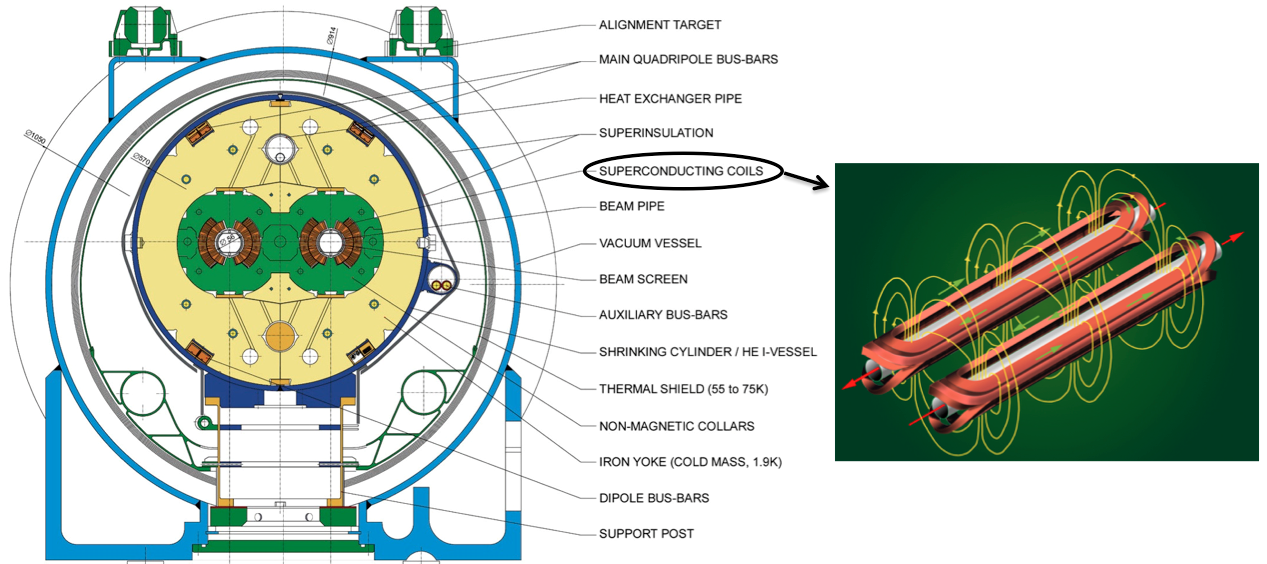
\includegraphics[scale=0.35]{figures/experiment/lhcdipole.png}
\caption[Dipole superconducting magnet]{Transverse section of the dipole superconducting coil and magnetic field induced by it \cite{Bruning:782076}.}
\label{dipole}
\end{figure}

The LHC circulates protons inside its beam-pipes in several very closely packed bunches, with each bunch made out of approximately 10$^{11}$ particles. To maximize the probability of the protons colliding with one another, the LHC squeezes the beam within a transverse size of $\sigma_x\approx\sigma_y\approx 15\,\mu$m.
\noindent Every 25 ns these bunches cross one another and several proton-proton collisions may take place, resulting in more than one interaction point per bunch crossing; this phenomenon is known as pileup. For instance, during the 2015 run at 13 TeV, there was in average 20 interactions per bunch crossing. 

The event rate (events/s) for a given process generated at the LHC is given by $\sigma_i \times {\cal L}$, where $\sigma_i$ is the cross section for the process under study and ${\cal L}$ is the instantaneous luminosity which depends only on beam parameters such as the number of particles per bunch ($n_1, n_2$), the revolution frequency ($f$) and the Gaussian widths of the beam profile in the horizontal and vertical plane ($\sigma_x\,,\sigma_y$):
\begin{equation}
{\cal L}  = f \frac{n_1 \, n_2}{4\pi \, \sigma_x \, \sigma_y}\,.
\end{equation}
The total number of events $N_i$ produced in a time $T$ is basically the integral of the event rate for the specific process, 
$\sigma_i \int^T_0 {\cal L} \, dt$.

\begin{figure}[p]
\centering
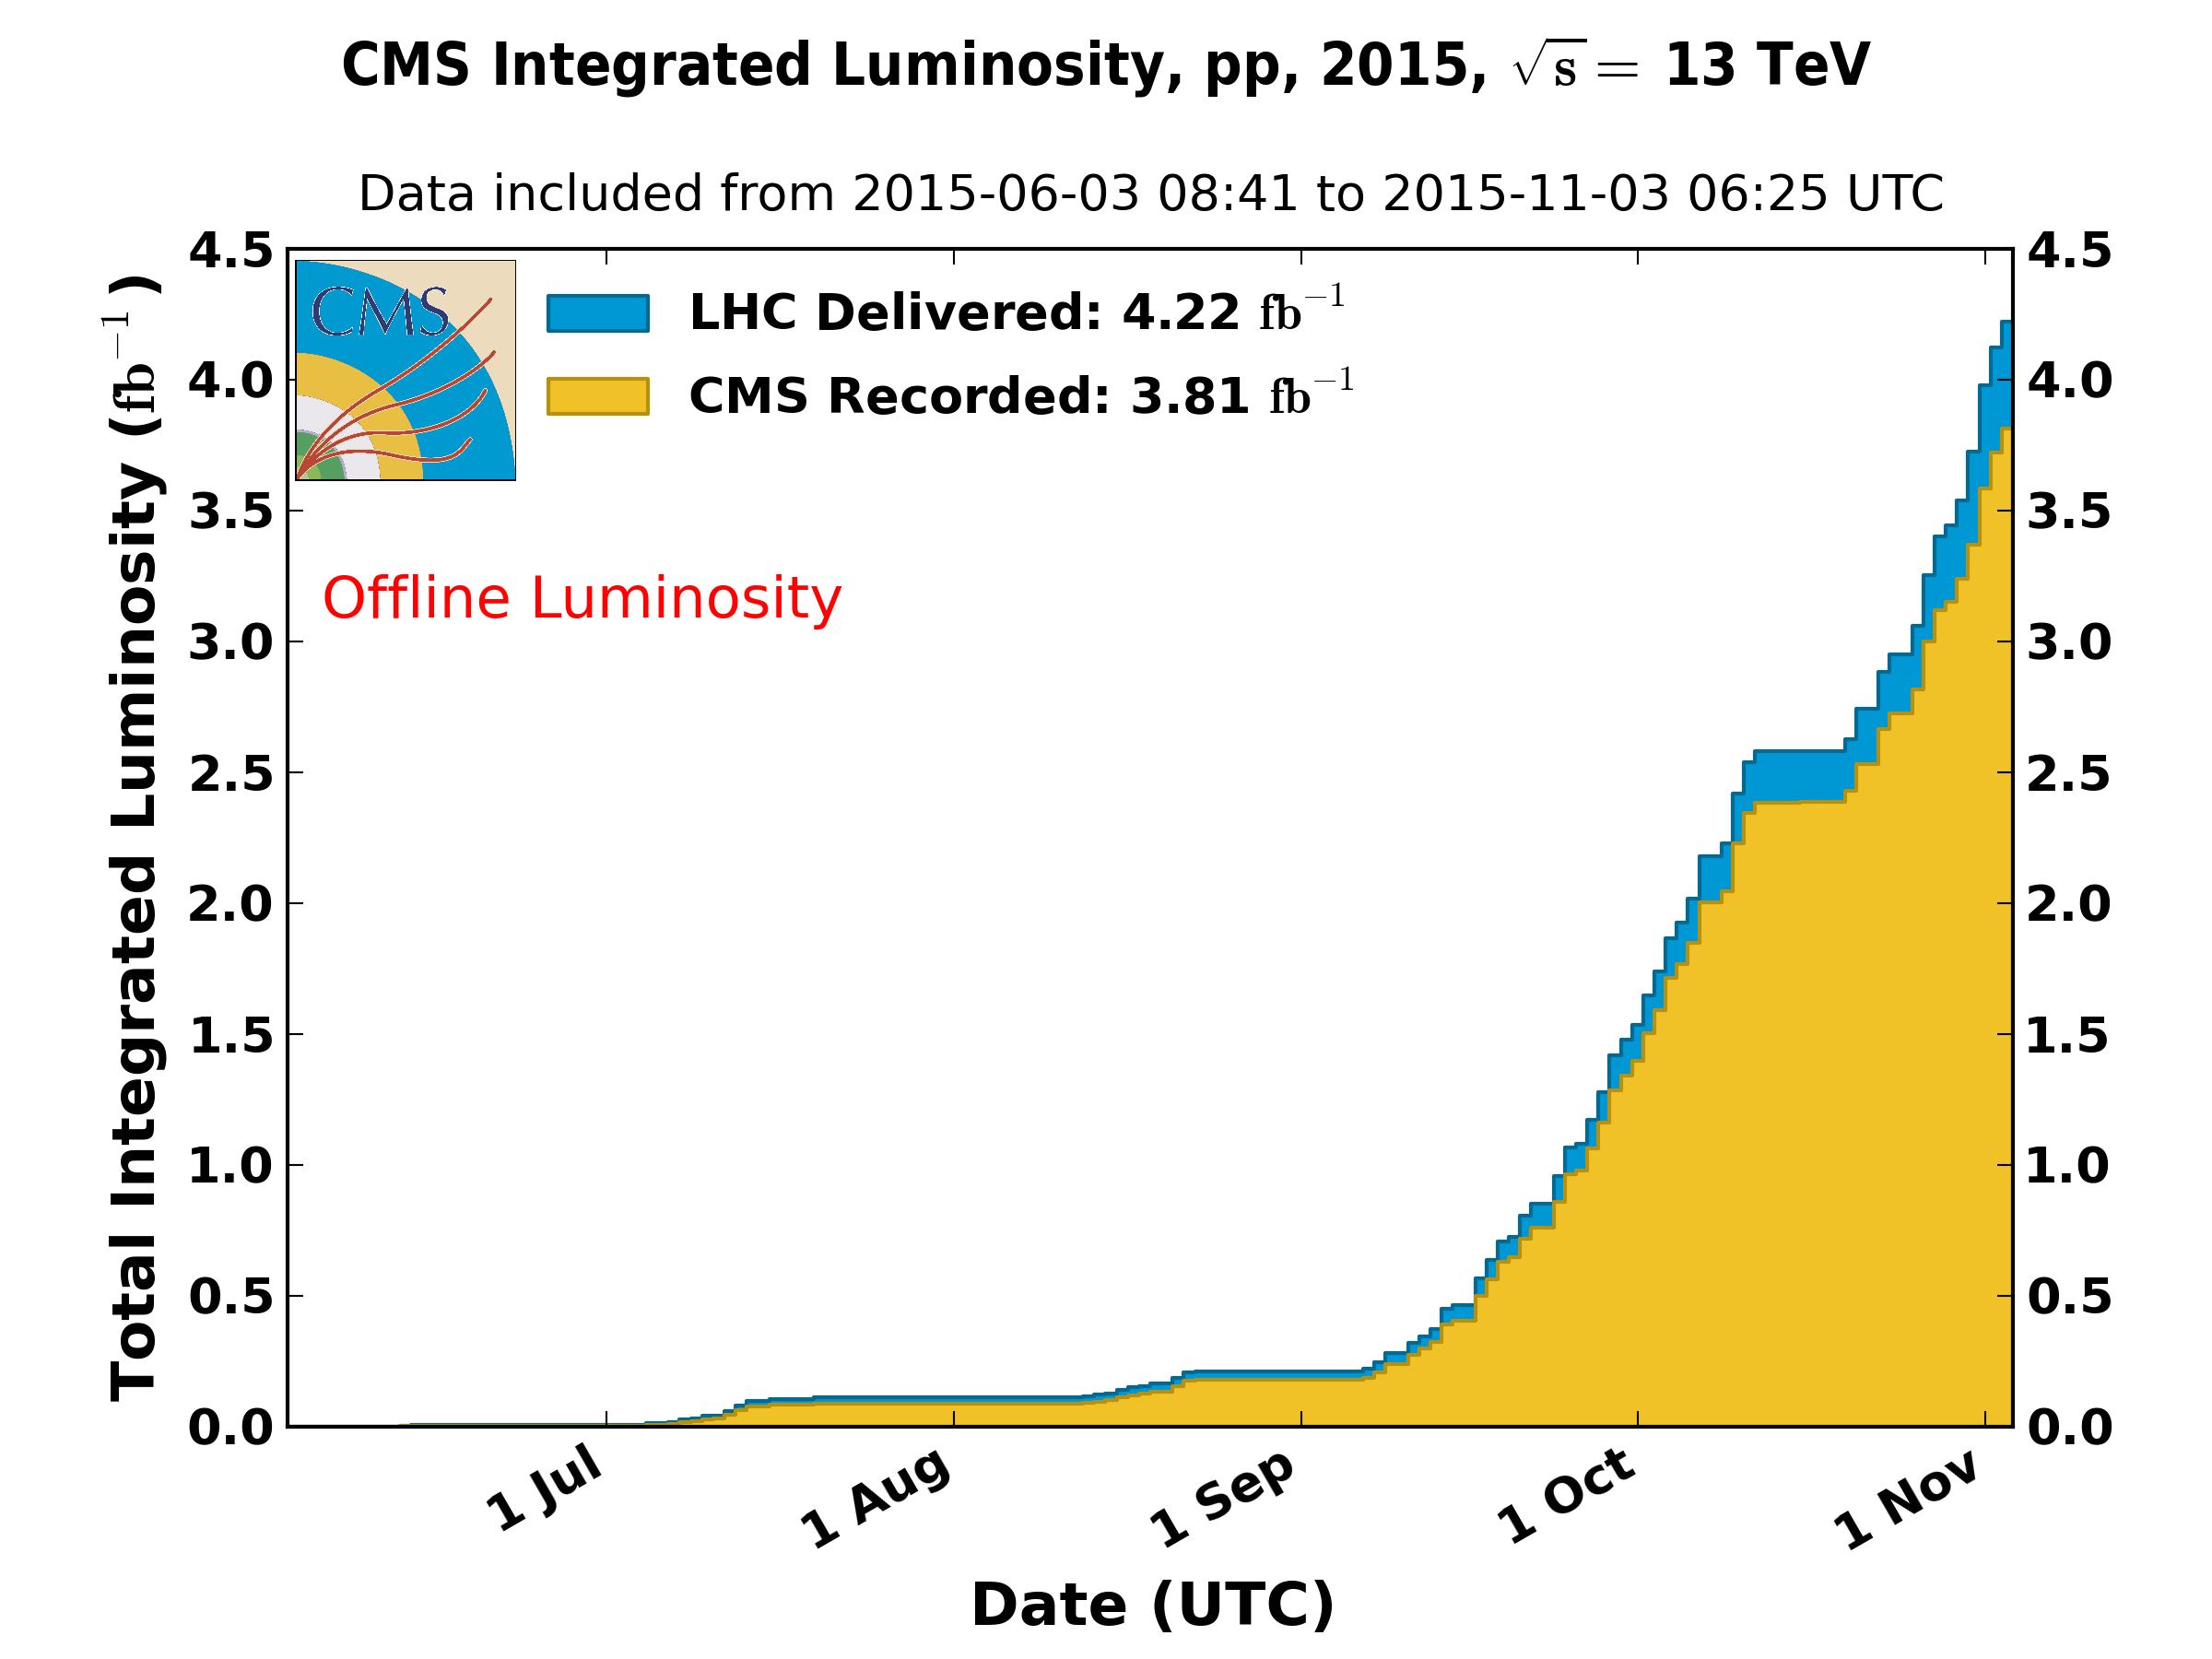
\includegraphics[scale=0.6]{figures/experiment/int_lumi_per_day_cumulative_pp_2015.png}\\\vspace{1cm}
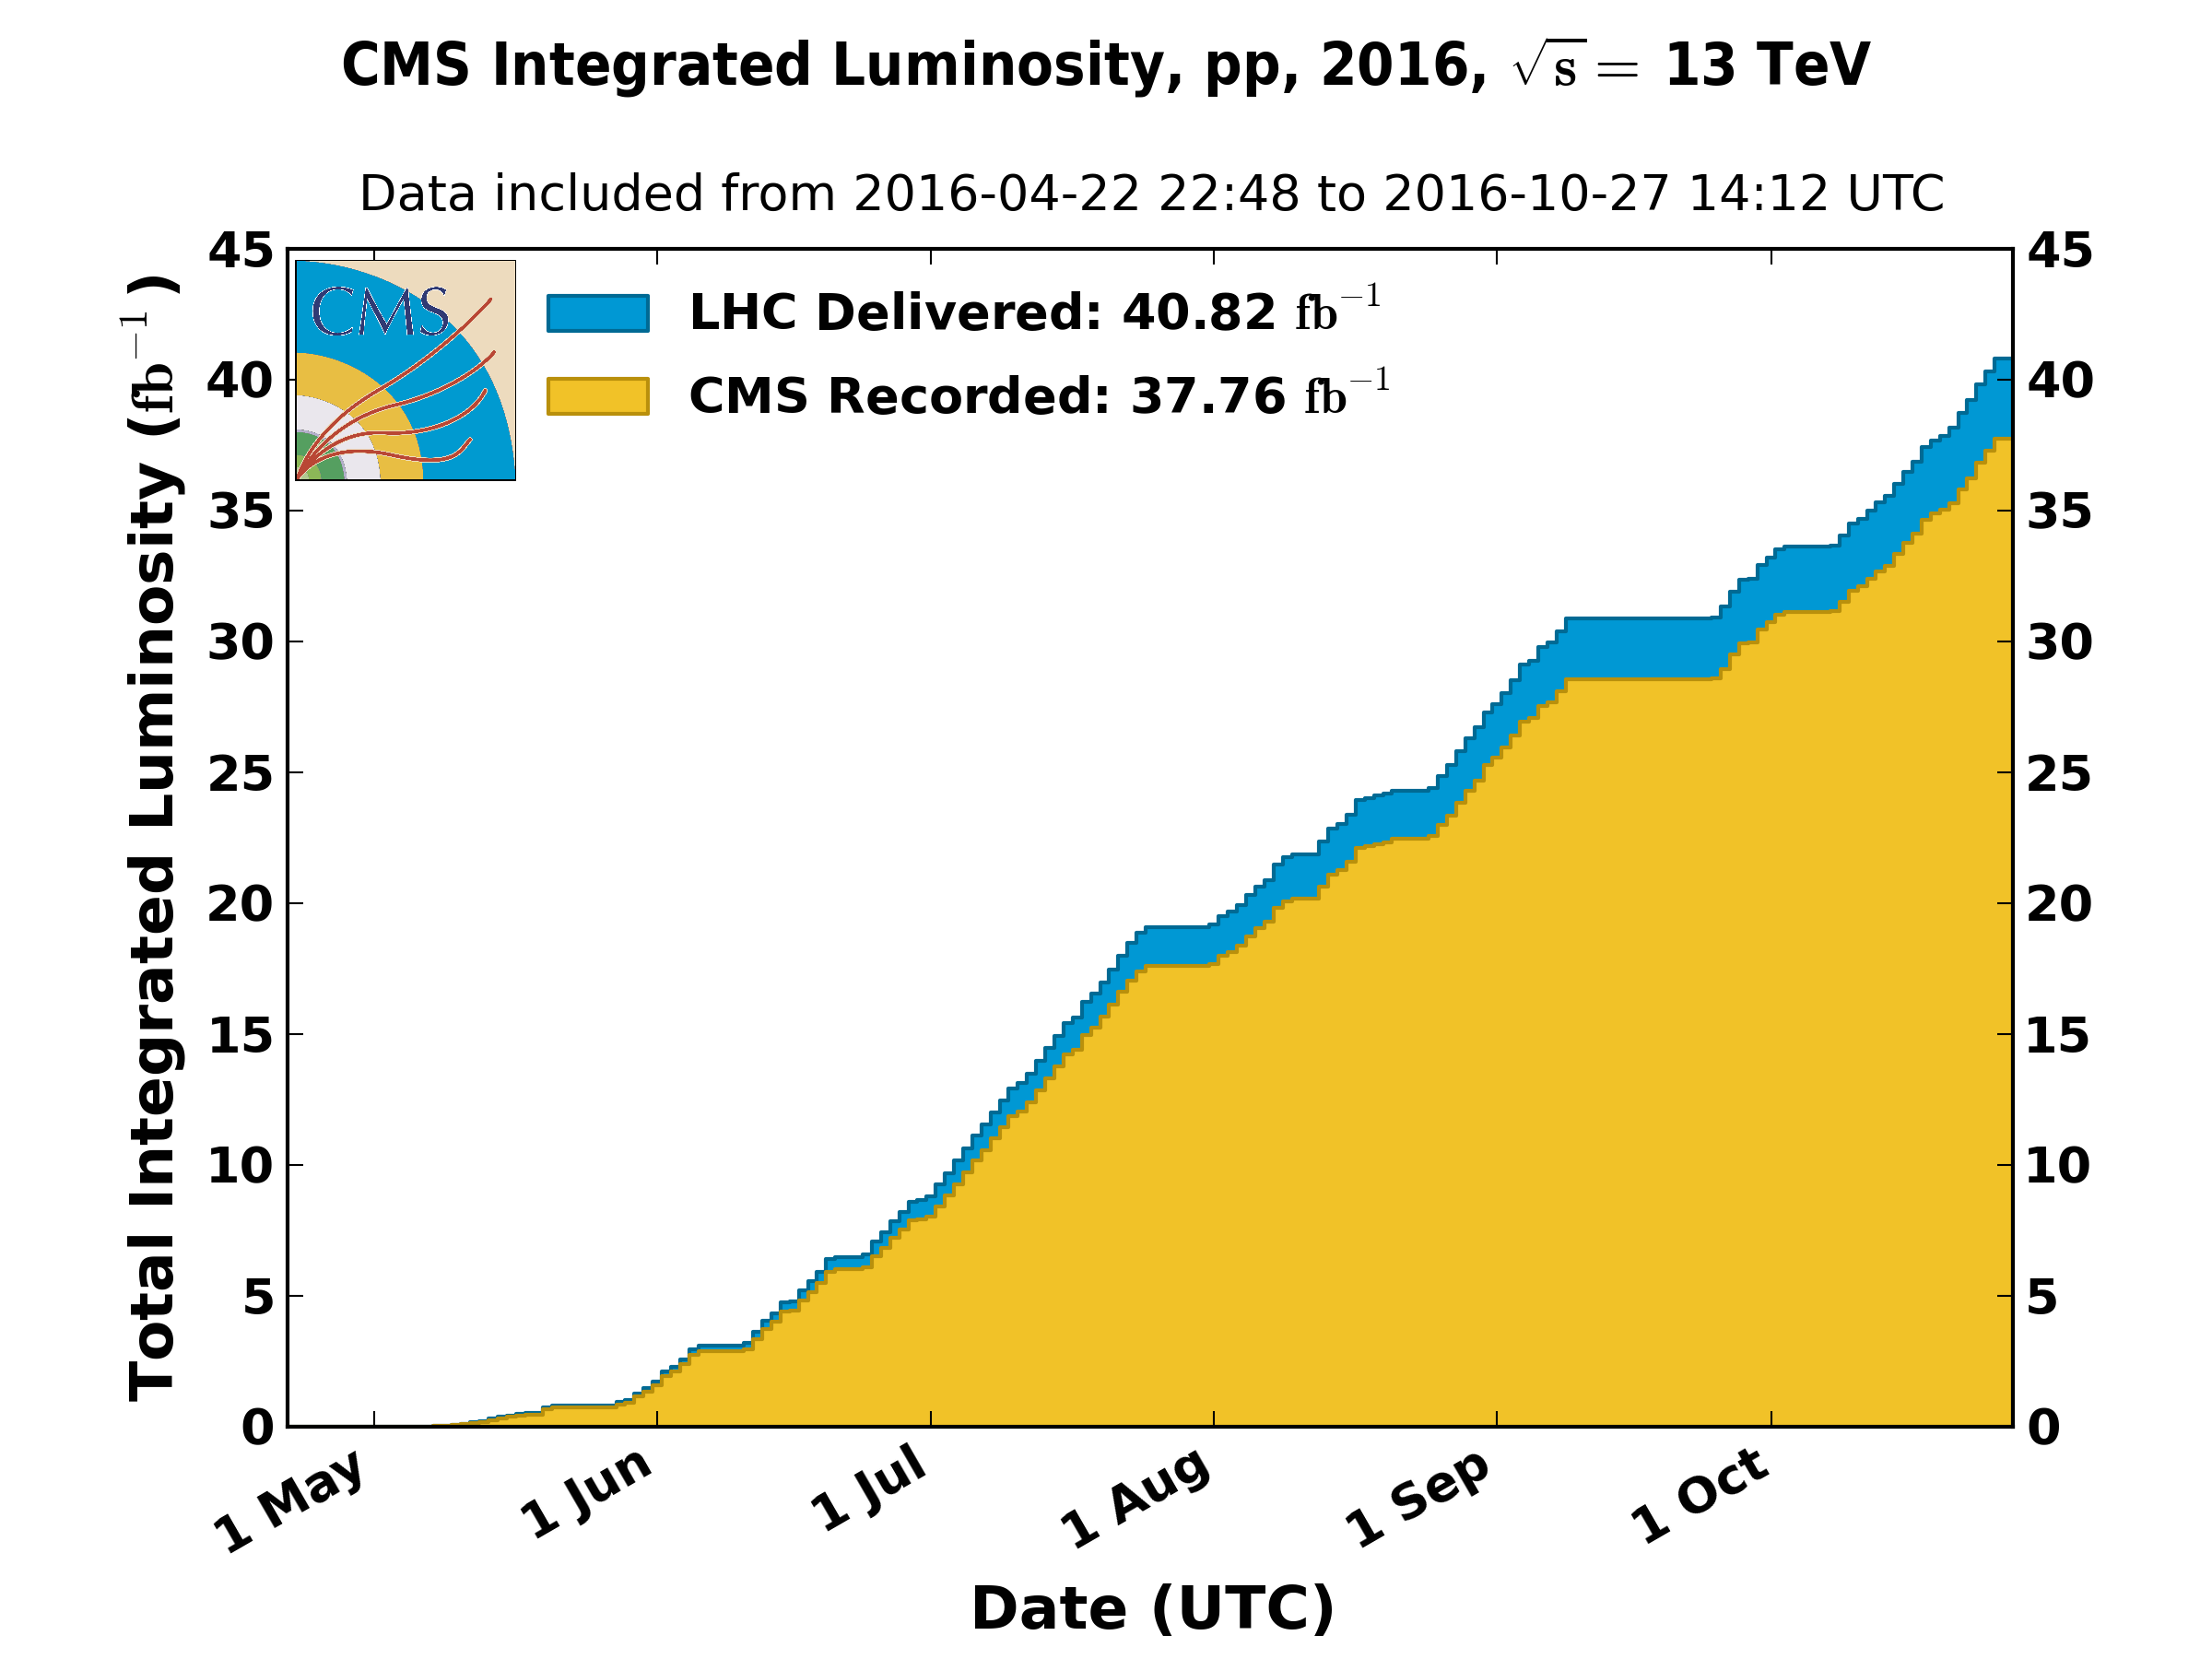
\includegraphics[scale=0.6]{figures/experiment/int_lumi_per_day_cumulative_pp_2016.png}
\caption[Performance of LHC over the Run 2]{Cumulative offline luminosity delivered by the LHC (blue) and recorded by CMS (orange) during stable beams and for p-p collisions at 13 TeV center-of-mass energy in 2015 (top) and 2016 (bottom) \cite{lumiPOG}.
} 
\label{lumiplot}
\end{figure}

The first collisions at the LHC took place in 2010 using proton beams with a center-of-mass energy of 7 TeV. In 2012 the center of mass energy was increased to 8 TeV and a further 23 fb$^{-1}$ of data were delivered. The next two years were dedicated to preparations for the LHC Run 2, ramping the center-of-mass energy up to 13 TeV. In 2015 the LHC delivered 4.2 fb$^{-1}$, and fantastically achieved \break 41.4 fb$^{-1}$ in 2016. The performance of LHC over the Run 2 is summarised in Fig. \ref{lumiplot}.

\section{The CMS Experiment}
The Compact Muon Solenoid (CMS) \cite{Bayatian:2006zz,Ball:2007zza} is one of the main experiments at the LHC. It is build around a solenoid magnet that takes the form of a cylindrical coil of superconducting cable that generates a field of 3.8 T. The bulk of the detector weights 12,500 tons and it is 21.6 meters long, 15 meters of diameter and 15 meters high.

% (Fig. \ref{CMSphoton}).
%\begin{figure}[h!!]
%\centering
%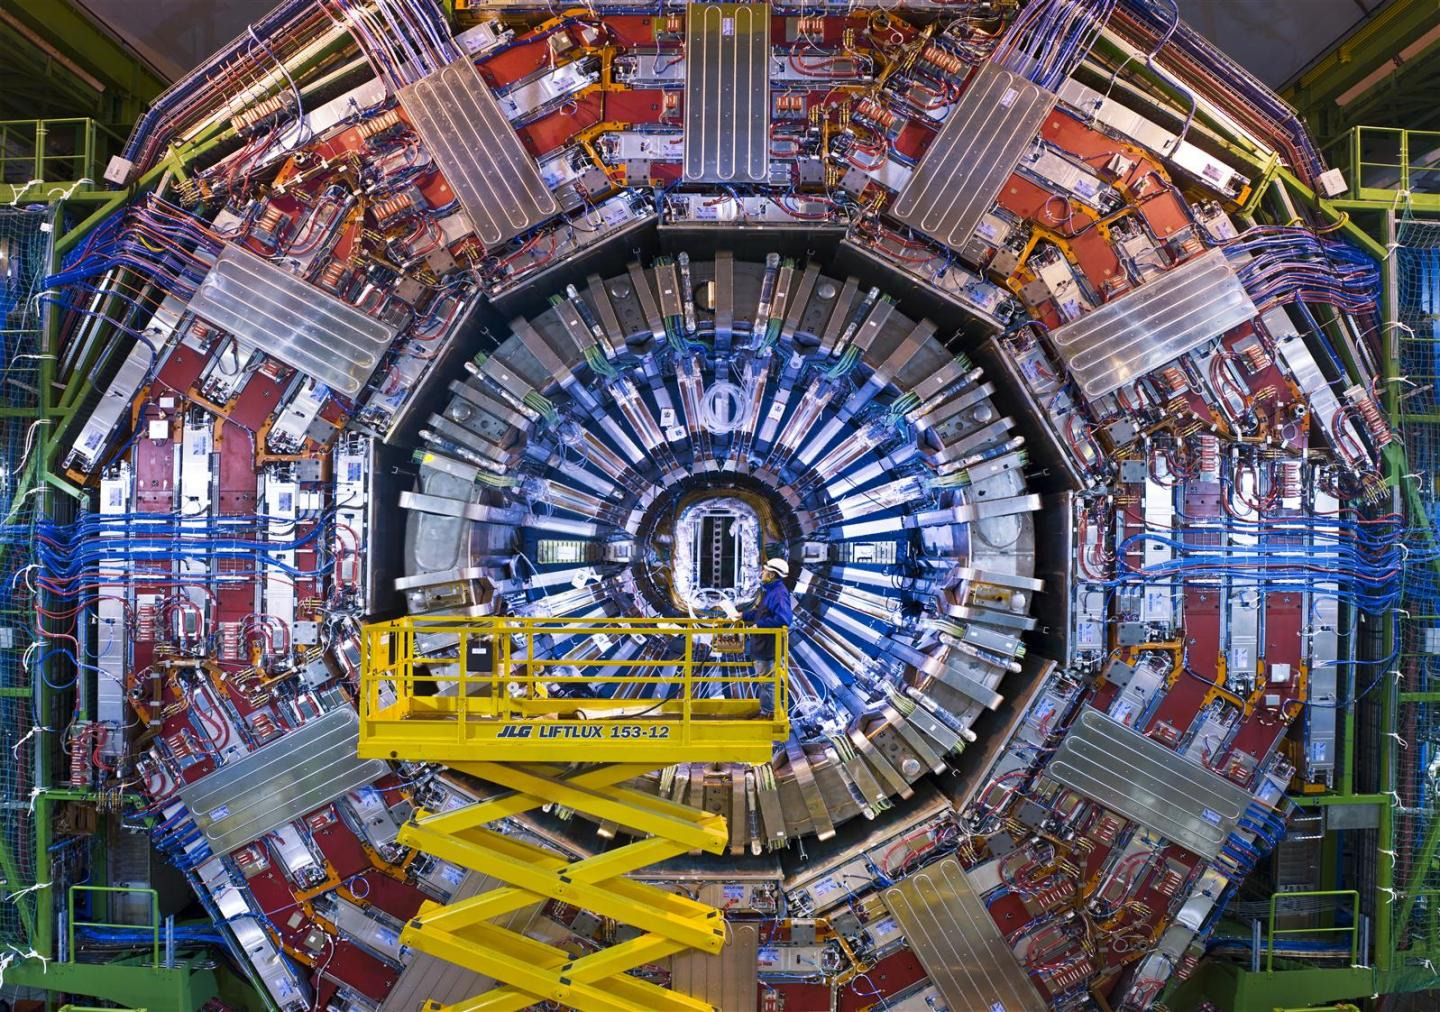
\includegraphics[scale=0.27]{figures/experiment/cms_0.jpeg}
%\vskip 1cm
%\caption[The CMS detector]{Transverse section of the barrel part of CMS \cite{CMS:1997263}.  }
%\label{CMSphoton}
%\end{figure}

% \newpage

CMS has a very compact design that emphasizes good muon identification. It provides good charge and momentum resolution including efficient $b$ and $\tau$ tagging capability as well as a good electromagnetic energy resolution and good missing transverse energy resolution. Contained within the superconducting solenoid volume are the silicon pixel and strip tracker, a lead tungstate crystal electromagnetic calorimeter (ECAL), and a brass and scintillator hadron calorimeter (HCAL). Muons are measured in gas-ionization detectors embedded in the steel flux-return yoke outside the solenoid. These sub-detectors are situated in an shell arrangement, and all the barrel systems have a forward equivalent to guarantee a 4$\pi$ solid angle coverage. Studying the layout in Fig. \ref{CMSlayout} more closely, one can observe additional very forward structures (muon detectors and a forward sampling calorimeter) to cover a high $|\eta|$ range. 

The identification of individual particle takes information from the various elements of the CMS detector. The energy of photons is directly obtained from the ECAL measurements, while the energy of electrons is determined from a combination of the electron momentum at the primary interaction vertex as determined by the tracker, the energy of the corresponding ECAL cluster, and the energy sum of the associated bremsstrahlung photons. The energy of muons is obtained from the curvature of the muon of the corresponding track. The energy of charged hadrons is determined from a combination of their momentum measured in the tracker and the matching ECAL and HCAL energy deposits. Finally, the energy of neutral hadrons is obtained from the corresponding ECAL and HCAL energy deposition.

\begin{figure}[h]
\centering
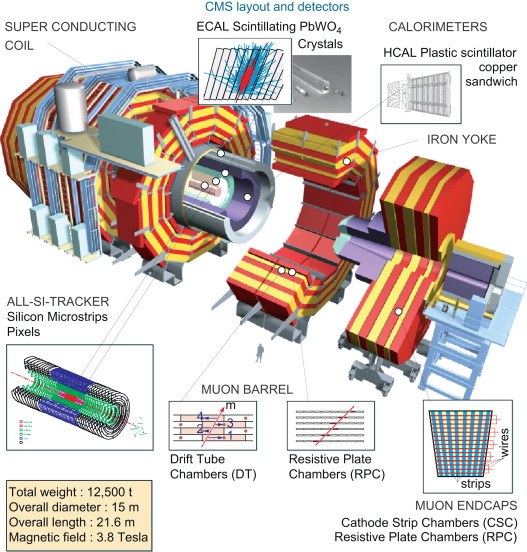
\includegraphics[scale=1.1]{figures/experiment/cmsLayout.jpg}
\vskip 1cm
\caption[The CMS detector and its components]{The CMS detector and its components \cite{CMS:1997263}.}
\label{CMSlayout}
\end{figure}

CMS uses a right handed coordinate system centered at the nominal collision point in which the  $+x$ axis points towards the center of the LHC ring, $y$ points up, and $+z$ points along the direction of the beam. In a cylindrical system $r$ is the radius from the nominal beam line and $\phi$ is the azimuthal angle. The pseudorapidity is defined as $\eta = -\ln [\tan(\theta/2) ]$, where $\theta$ is the polar angle measured from the $+z$ axis. The transverse momentum is defined as $\ptrans=p\cdot\sin\theta$, with $p$ being the particle momentum.

\section{Main Detector Components}

\subsection{Tracker System}
The tracker system comprises two components: the pixel detector and the silicon strip detector. The pixel detector is the innermost subsystem, closest to the beam pipe, containing 66 million of $100\times150\,\mu {\rm m}^2$ pixels responsible for track reconstruction and primary vertex identification as well as $b$ tagging. It is arranged in three barrel layers and two endcap disks at each end. The pixel detector is followed by a silicon strip system, which determines the momentum of electrically charged particles that traverse it. The system is structured in ten barrel layers and twelve endcap disks, composed of 9.6 million strips with pitch between 80 and 180 $\mu$m, with a total silicon surface area of 200 m$^2$. 

After the first years of CMS operations, there was an upgrade proposal \cite{Dominguez:1481838} to replace the pixel detector for a new high efficiency and low mass detector including four barrel layer and three forward/backward disks. The new pixel was just installed and the commissioning is currently ongoing, being 2017 the first year to include this important upgrade.  

\subsection{Electromagnetic Calorimeter}
The tracker is followed by an Electromagnetic Calorimeter (ECAL), which uses 75,000 lead tungstate (PbWO$_4$) crystals to determine the energy of electrons and photons, producing an amount of light that is proportional to the particle's energy. The ECAL is distributed in a barrel ($|\eta| < 1.479$) and two endcap ($1.479 < |\eta| <3.0$) regions. Photodetectors placed in the back of each crystal detect the scintillation light and convert it to electrical signals. Electromagnetic showers are very narrow in lead tungstate helping particle identification and the implementation of isolation criteria. Figure \ref{cmsEcal} shows a transverse section of the ECAL. 

Pre-shower detectors consisting of two planes of lead followed by silicon sensors are located in front of the endcaps. When a photon passes through the lead layer it causes an electromagnetic shower containing electron-positron pairs, which are detected by the silicon sensors. From this the photon's energy is measured, whilst having two detector layers gives the particle's position. The preshower has a much finer granularity than the ECAL, with detector strips 2 mm wide compared to the 3 cm-wide ECAL crystals, what allows to distinguished closely-spaced photons. 

\begin{figure}[h!!]
\centering
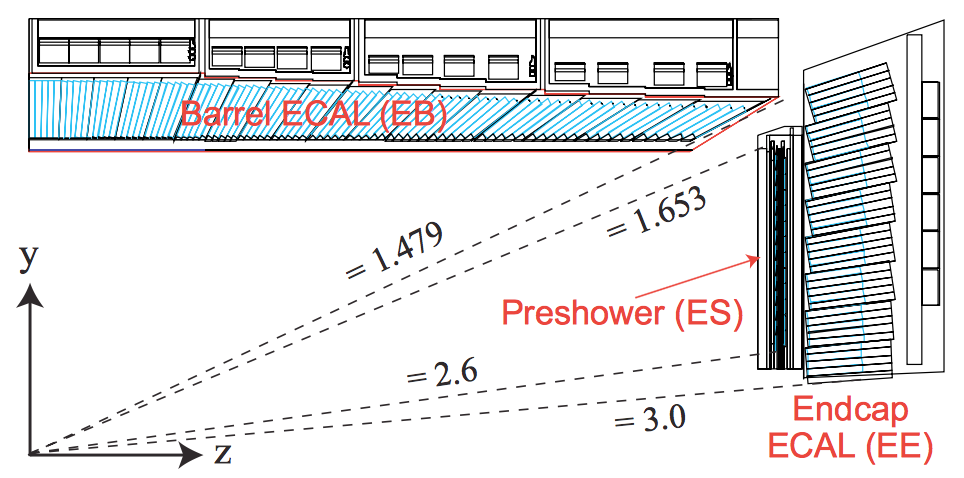
\includegraphics[scale=0.35]{figures/experiment/cmsEcal.png}
\vskip 1cm
\caption[CMS ECAL]{Transverse section through the ECAL \cite{Bayatian:2006zz}.}
\label{cmsEcal}
\end{figure}

\subsection{Hadronic Calorimeter}
The ECAL is surrounded by a brass/scintillator sampling Hadron Calorimeter (HCAL) to measure the energy of hadrons. Optical fibers collect up the light produced by the plastic scintillators and feed it into readout boxes where photodetectors amplify the signal. The HCAL covers the region with $|\eta|<3.0$. Their thickness varies from 7 to 10 interaction lengths depending on $\eta$; a scintillator placed outside of the coil at the innermost muon detector extends the instrument thickness to more than 10 interaction lengths everywhere. Quartz fibre and iron forward calorimeters, read out by photomultipliers, extend the calorimeter coverage in the range $3.0 < |\eta| < 5.0$ comprising the hadron endcap (HE) and hadron forward (HF) calorimeters.

\subsection{Solenoid}
The central feature of the CMS apparatus is a 13 m long and 6 m diameter superconducting solenoid, providing a magnetic field of 3.8 T. Within the field volume are the tracker system and the calorimeters. The magnet bending power ensures the unambiguous determination of the sign for muons with a momentum of $p \approx$ 1 TeV, providing a momentum resolution of $\Delta p / p \approx 10 \%$.

\subsection{Muon System}
Outside the solenoid is the muon system, the most visible part of CMS shown in Fig. \ref{muoneta}. The CMS design relies on the high bending and excellent muon momentum resolution, which uses an iron return yoke interleaved with the muon chambers to increase the magnetic field. With the field parallel to the LHC beam axis, the muon tracks are bent in the transverse plane. 

\begin{figure}[p]
\centering
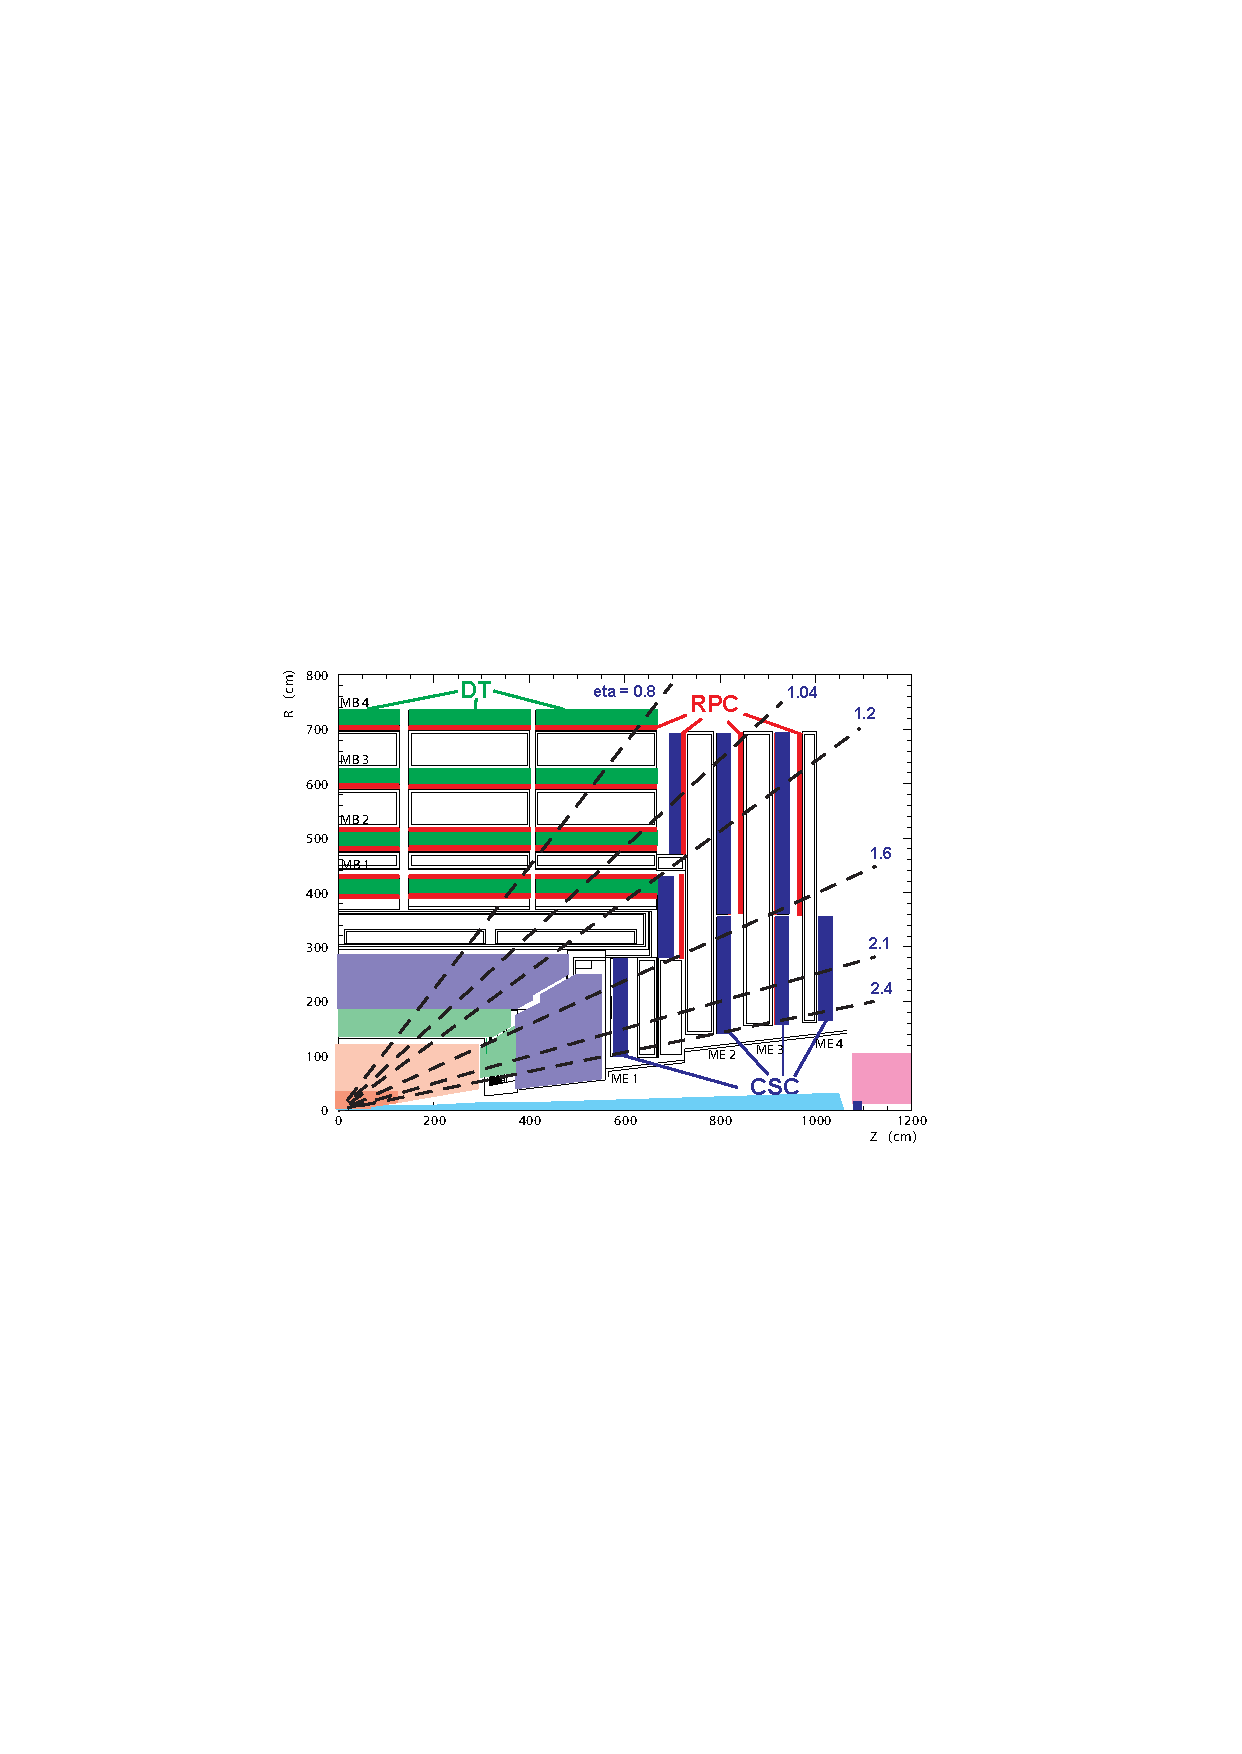
\includegraphics[scale=1.1]{figures/experiment/muonDetectors_eta.pdf}\\
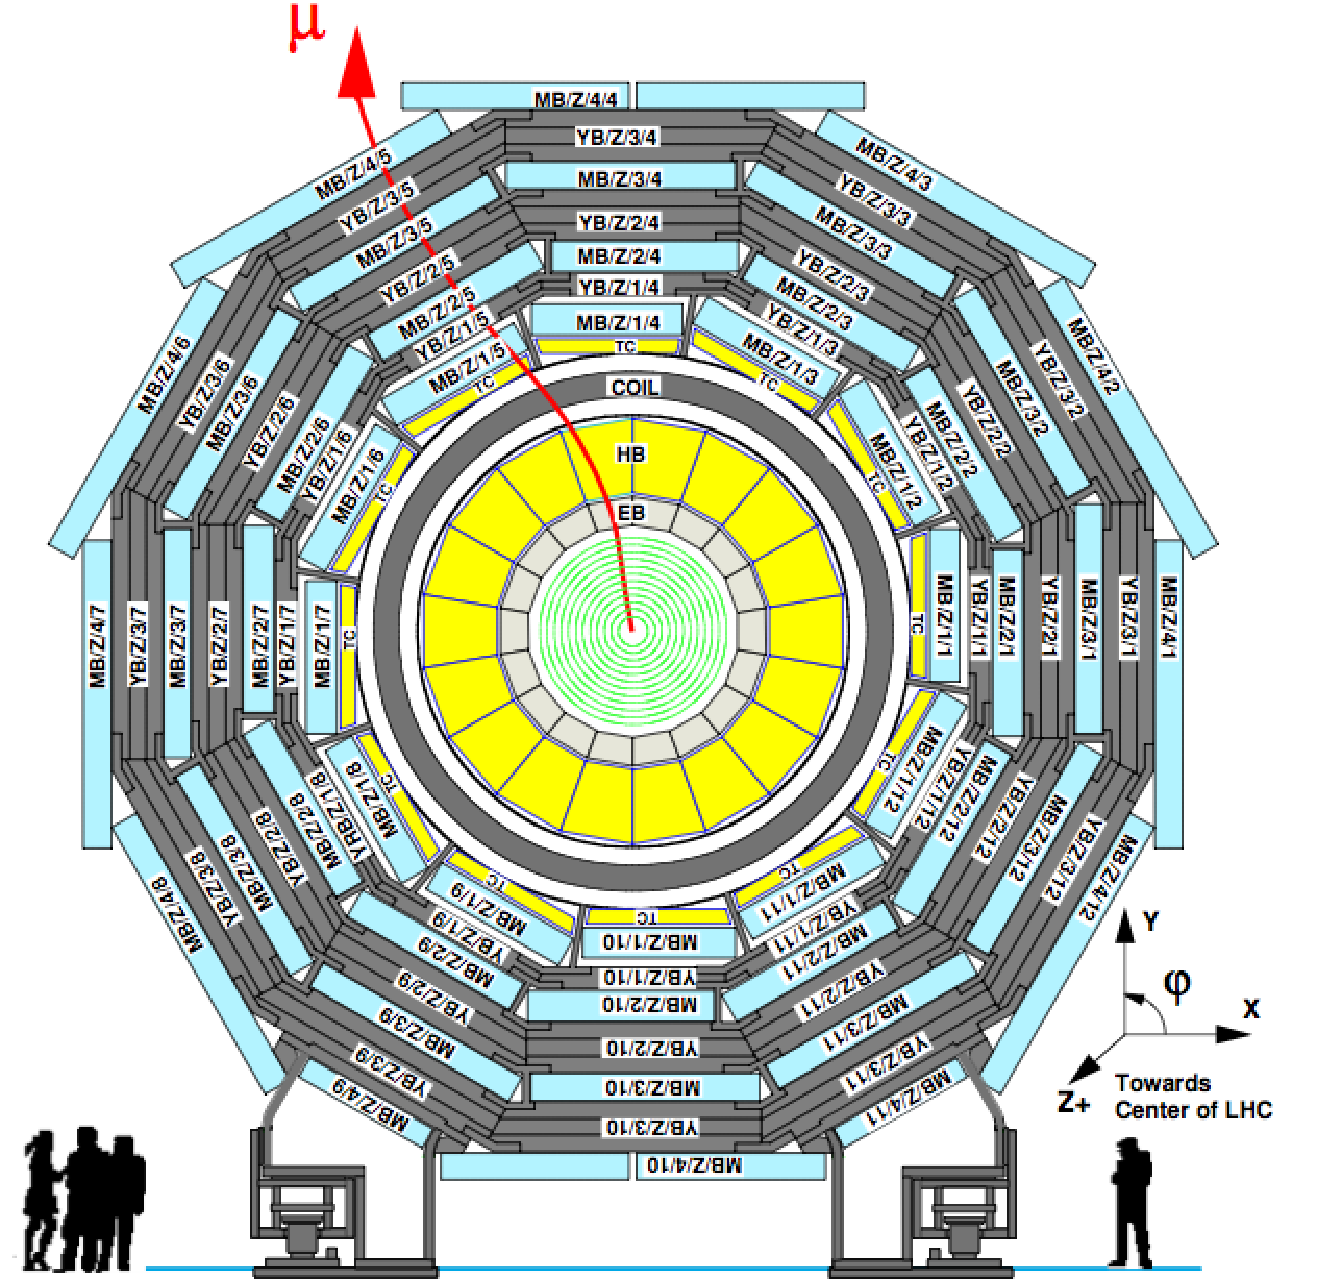
\includegraphics[scale=0.5]{figures/experiment/DT1.pdf}
\caption[Pseudorapidity coverage of the muon system]{Pseudorapidity coverage of the muon system (top) and muon track in the transverse plane (bottom).}
\label{muoneta}
\end{figure}

The iron yoke is instrumented with aluminum Drift Tubes (DT) in the barrel ($|\eta| < 1.2$) and Cathode Strip Chambers (CSC) in the end-cap region ($0.9<|\eta|<2.4$). Due to the iron yoke, the momentum resolution of the CMS muon system is dominated by the multiple scattering. The standalone muon momentum resolution is $\sigma(\ptrans)/\ptrans=9\%$ for $\ptrans\le 200$ GeV/$c$ and 15--40\% at $\ptrans=1$ TeV/$c$, depending on $\eta$. Including the tracking system improves the result by an order of magnitude for low momenta. At 1 TeV the contribution of both measurements lead to a momentum resolution of about 5\%. 

The DT and CSC subsystems can each trigger on muons with large transverse momentum in the range $|\eta|<2.4$. However, for the full LHC luminosity, faster trigger chambers are needed to associate the detected muons to the right crossing of proton bunches. Resistive Plate Chambers (RPCs) covering the region $|\eta|<1.6$ are used by the muon system for fast trigger.

\subsection{Trigger and Data Acquisition}
The CMS online systems need to select around 1 kHz of interesting events out of a rate of 40 MHz. The event selection is done with two trigger levels: the level 1 trigger \cite{Dasu:2000ge}, based on custom electronics, reduces the rate to 100 kHz. The data acquisition (DAQ) system \cite{Sphicas:2002gg, Bawej:2015tmz} reads out the detector and passes the events to the high-level trigger, a software system based on the full CMS reconstruction software running on a farm of computers. The CMS DAQ system was designed to handle a throughput of 100 GB/s, making it the highest throughput DAQ system in high energy physics to date.

%\clearpage
\section{Identification of Physical Objects}
The identification of stable particles in CMS relies on the different interactions of a particle with the sub-detectors. While photons, electrons and hadrons lose most of their energy and are stopped in the calorimeters, muons deposit only a small fraction of their energy through ionization so they reach the outer part of the detector, where the muon chambers are located. These characteristic signatures (Fig. \ref{PId}) based on tracking and calorimetry are crucial aspects for particle identification.

The sub-detectors in CMS are stacked in radial layers and a particle passes through these layers sequentially from the collision point outward: first the tracking system, then the electromagnetic and hadronic calorimeters, finally the muon system. All layers are embedded in a magnetic field in order to bend the tracks of charged particles for momentum and charge sign determination.

\begin{figure}[htb!!!]
\centering
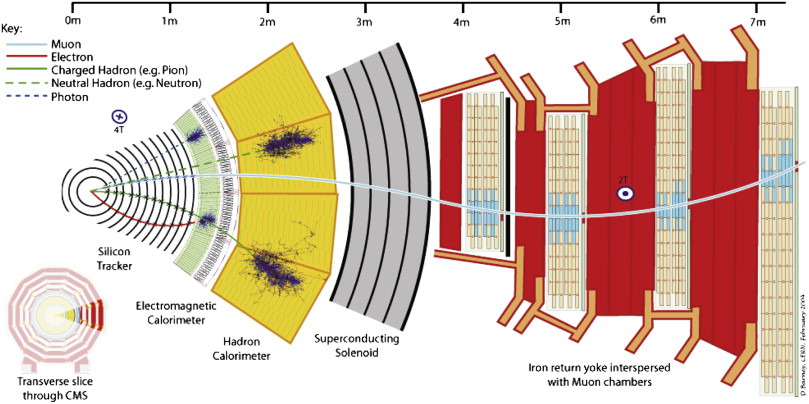
\includegraphics[scale=1.15, angle=90]{figures/experiment/CMSPId.jpg} 
\caption[Characteristic signatures of different particles in CMS]{Characteristic signatures of different particles in CMS.}
\label{PId}
\end{figure}

\subsection{Track Reconstruction}
The track reconstruction uses an iterative procedure \cite{Khachatryan:2010pw} consisting of a number of steps to select the better tracks first; the hits associated with the first tracks are removed, and then, other tracks are reconstructed from the remaining hits. 

Each of the tracking steps starts with a collection of seeds formed from 2 (a pair seed) or 3 (a triplet seed) pixel hits consistent with some minimum track $\ptrans$, and coming from some region of the beam spot. The first steps use triplet seeds and higher minimum track $\ptrans$, these are followed by steps using pair seeds and lower $\ptrans$. The later steps use seeds that contain hits from the silicon strip detector to find detached tracks, \textit{e.g.} from decay products of $K^0_s$ mesons or $\Lambda^0$ baryons. 

\subsection{Primary Vertex Reconstruction} 
CMS observes the decay products of various particles produced and work backwards to determine which collision interactions produced which particles. In the CMS tracker (made up of silicon pixels and strips), the number of hits grows linearly with pileup. As these hits need to be combined into tracks, the number of possible combinations that make a track grows fast with pileup. Fortunately, the high granularity and efficiency of the tracker provides the means to distinguish the many tracks in an event. An illustration of the CMS tracking capabilities is shown in Fig. \ref{pileup}; the figure diplays the reconstructed tracks and the primary vertices in a real event recorded on 2016-Oct-14, during the proton-proton collisions at 13 TeV delivered by the LHC. 
\begin{figure}[ht]
\centering
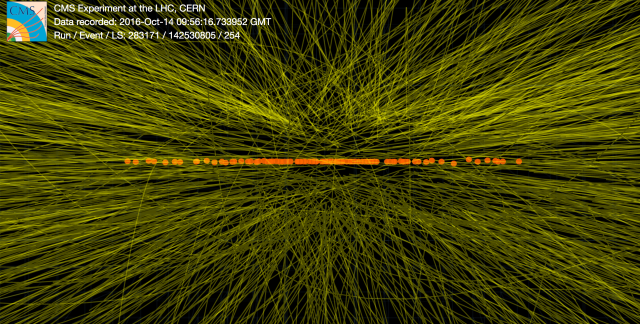
\includegraphics[scale=1.34]{figures/experiment/highpileup.png} 
\caption[Tracks in a typical collision]{Tracks and primary vertices as seen in a typical collision \cite{McCauley:2231915}.}
\label{pileup}
\end{figure}

The vertex reconstruction can be seen as a clustering procedure in which each vertex is a cluster of tracks selected by a fitting algorithm. Among the algorithms used in CMS for vertex fitting are the Kalman filter (KVF) \cite{Fruhwirth:1991pm}, and the Adaptive Vertex Fitter (AVF) \cite{Fruhwirth:2003xw}. The Kalman filter is a least-squares estimator which minimizes the sum of the squared distances of all tracks from the vertex position. The AVF algorithm is formulated as an iterative re-weighted Kalman filter, associating a weight $w_i$ interpreted as the probability that track $i$ belongs to a vertex. The AVF algorithm is a robustification of the Kalman filter to deal with fitting errors, such as mis-associated tracks or mis-measured track errors.

\subsection{Jet Reconstruction}
\label{JetSection}
Hadronic jets are the experimental signatures of quarks and gluons (Fig. \ref{jets}). In CMS, jets are clustered with the anti-$k_T$ algorithm \cite{Cacciari:2008gp} starting from a collection of particle-flow (PF) candidates \cite{CMS:2009nxa,CMS:2010byl}. A correction based on the projected area of the jet on the front face of the calorimeter is used to take into account the extra energy due to neutral particles coming from pileup.  

The particle-flow (PF) algorithm integrates measurements from all components of the CMS detector in order to reconstruct a complete list of candidates per event, including muons, electrons, photons, charge and neutral hadrons. The jet clusterization routine loops over the list of PF candidates, and recombines two particles $i$ and $j$ based on the condition $d_{ij} < k_{ti}^{2p}$, where the distance $d_{ij}$ is defined as: 
\begin{equation}
	d_{ij} = \min(k_{ti}^{2p}, k_{tj}^{2p}) \frac{(\eta_i - \eta_j)^2 + (\phi_i - \phi_j)^2}{R^2}.
\end{equation}
The transverse momentum, pseudo-rapidity, and azimuth angle of particle $i$, are $k_{ti}$, $\eta_i$, and $\phi_i$, respectively. The parameter $p=-1$ is characteristic of the anti-$k_T$ algorithm \cite{Cacciari:2008gp}, and ensures infrared-safe jets. The aperture of the jet is controlled with the parameter $R$, which takes the value $R=0.8$ for the case of merged jets; the number $R=0.8$ is set by the CMS jet study group \cite{Khachatryan:2014vla}, and it is kept fix along the jet reconstruction routine for both data and simulation.

\begin{figure}[ht]
\centering
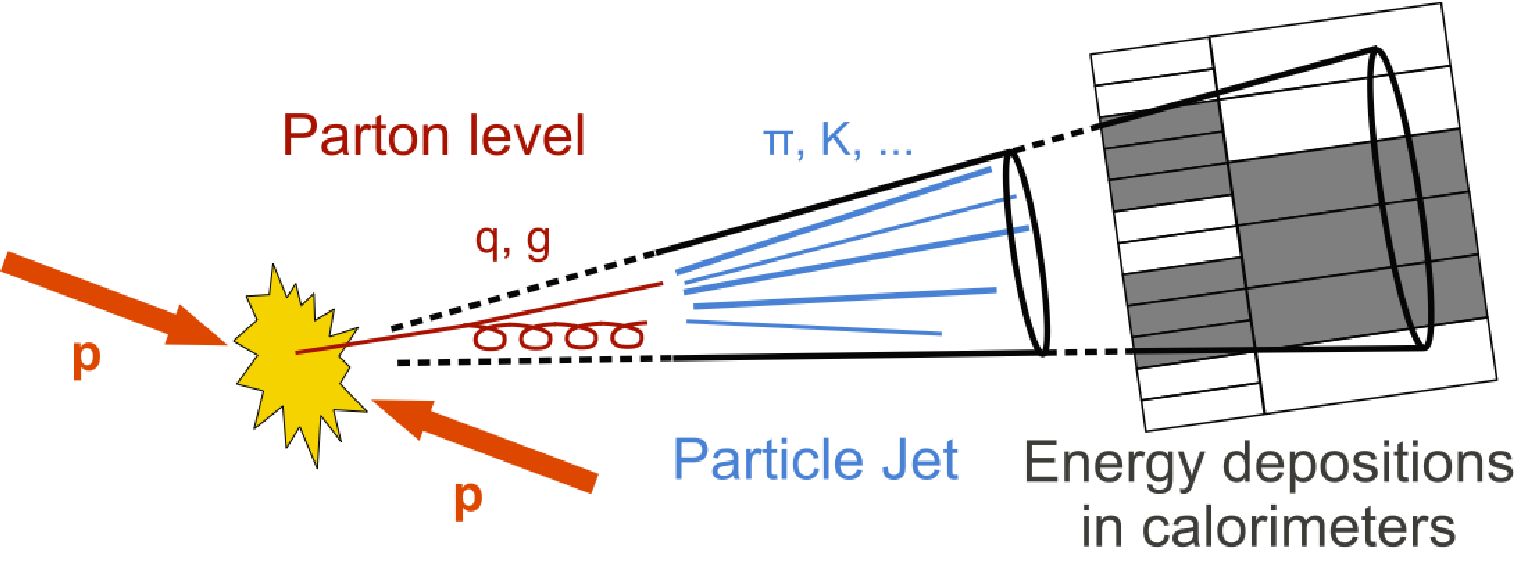
\includegraphics[scale=0.22]{figures/experiment/CaloJet.png} 
\caption[Collimated spray of particles]{Schematic production of a hadronic jet.}
\label{jets}
\end{figure}

Hadronically decaying W and Z bosons are identified as jets with distance parameter $R=0.8$. In order to discriminate W/Z jet candidates against multijet backgrounds, the reconstructed jet mass is required to be close to the W or Z boson mass, in addition to require a two-prong jet substructure produced by the initial quarks. Jets coming from the merged decay products of a single V boson are usually referred as V jets. 

Different jet grooming algorithms have been explored in CMS and their performance in multijet processes has been studied in detail \cite{Chatrchyan:2013vbb}. The goal of jet grooming is the elimination of soft, large-angle QCD radiation that increases the V jet mass compared to the initial V boson. Further discrimination is obtained from the quantity called N-subjettiness \cite{Thaler:2011gf} defined as
\begin{equation}
	\label{eq:tauN}
	\tau_N = \frac{1}{d_0} \sum_k{p_{T,k} \min(\Delta R_{1,k}, \Delta R_{2,k}, \cdots, \Delta R_{N,k})}\,, 
\end{equation}
where the index $k$ runs over the jet constituents and the distances $\Delta R_{n,k}$ are calculated with respect to the axis of the $n$th subjet. The normalization factor $d_0$ is calculated as $d_0 = \sum_k{p_{T,k}R_0}$, setting $R_0$ to the radius of the original jet. 

\begin{figure}[h]
\centering
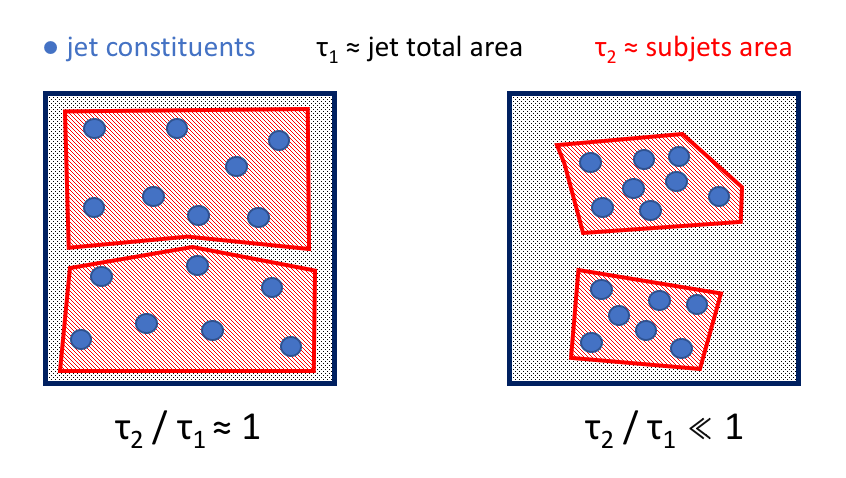
\includegraphics[scale=0.35]{figures/experiment/visualTau21.png} 
\caption[Intuition of Tau21]{Schematic representation of the N-subjettiness discriminant. A two-prong jet substructure produces lower values of the ratio $\tau_2/\tau_1$.}
\label{visualtau21}
\end{figure}

The variable $\tau_N$ quantifies the capability of clustering the jet constituents in exactly $N$ subjets. The ratio $\tau_{21} = \tau_2 / \tau_1$ is actually a powerful discriminant between jets originating from hadronic V decays and from gluon and single-quark hadronization. Jets coming from hadronic W or Z decays are characterized by lower values of $\tau_{21}$, given the two-prong substructure adopted by the jet constituents schematically depicted in Fig. \ref{visualtau21}. The visual representation in the above figure has to be taken with a grain of salt, since the definition of $\tau_N$ (Eq. \ref{eq:tauN}) depends on the kinematic properties of the jet constituents, rather than the jet area.

\subsection{Missing Energy}

Neutrinos produced in the final state, as well as other hypothetical weakly interactive neutral particles, escape from the detector causing an energy imbalance in the observed event. Momentum conservation is the available way to reveal the presence of neutrinos. 

\begin{figure}[h]
\centering
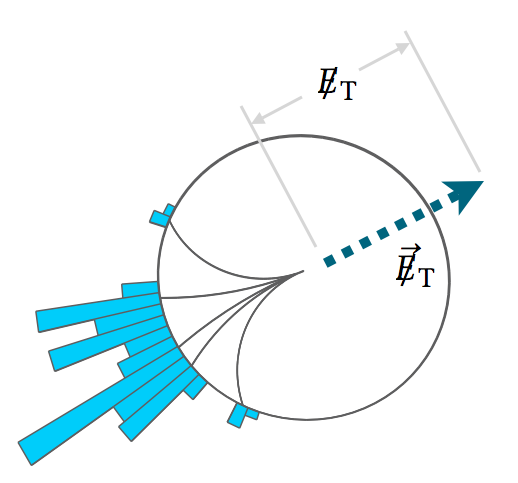
\includegraphics[scale=0.4]{figures/experiment/metFig.png} 
\caption[Missing transverse momentum and its magnitude]{Missing transverse momentum and its magnitude.}
\label{missing}
\end{figure}


Since the $z$-component of the momentum of the colliding partons is not known, one cannot determine the net missing energy caused by neutrinos. However, the total momentum in the transverse plane is zero to a very good approximation. 

One can define the missing transverse momentum as the negative vector sum of the transverse energies of all final-state particles reconstructed in the detector. The missing transverse energy $\met$ corresponds to the magnitude of the missing transverse momentum (Fig. \ref{missing}).  
\begin{equation}
\vec{\met} = -\sum_i \vec{\etrans}^i
\end{equation} 


\section{Software and Computing}
The Monte Carlo (MC) method is a numerical technique for calculating probabilities and related quantities by using sequences of random numbers. The MC technique is appropriate to simulate physical events, since the randomness of the MC method allows to capture the uncertainty that is present in most physical measurements. 

Of great interest in physics are the MC event generators, they include matrix element calculators like AlpGen \cite{Mangano:2002ea}, MadGraph \cite{Maltoni:2002qb}, and multi-purpose MC generator like PYTHIA \cite{Sjostrand:2007gs}. Matrix element calculators deliver an event at the parton level, then MC generators can further be used to develop a fully hadronized event. 

PYTHIA provides the generator level of what happens in a particle collision: implements models for a number of physics aspects, such as hard and soft interactions, parton distributions, initial and final state radiation, multiple interactions, fragmentation and decay, and hadronization of the parton-level events. However, the generation of events is only the first step in the complete analysis chain.

\subsection{Event Reconstruction}

The detailed simulation and reconstruction of physics events is extremely time consuming. The analysis chain is decomposed into four major steps as follows:
\begin{compact_enumerate}
\item {\it Generation of Monte Carlo events:}
The Monte Carlo events are created using generators like PYTHIA. These generators produce a list of particles and their four-vectors;
\item {\it Simulation of material effects:}
This is the most time consuming step. The output of this step is called \emph{SimHits}. They contain the information about the energy stored in different detector elements at different times;
\item {\it Simulation of readout electronics (digitalization):} 
The detector converts the energy deposited by the particles into electronic signals that are converted to digital information. Since the simulation of material effects requires large amount of CPU time, the minimum bias events are randomly selected from a large pool of simulated events and combined with the simulated signal events. The combination of minimum bias events with a signal event and the simulation of the detector response to the energy deposition are performed by the reconstruction software. The output created in this step is called \emph{DIGI};
\item {\it Reconstruction of physics/analysis objects: }
The reconstruction is performed in several sub-steps. First the \emph{DIGI} are combined to reconstructed hits \emph{RecHits}, which for example combine several strips of the silicon tracking detectors. Then \emph{RecHits} are used to find tracks in the inner tracker and the muon chambers and clusters in the calorimeters. The reconstruction can produce more complicated objects like jets or information about the missing energy and finally physical objects like electrons, photons, muons etc. 
\end{compact_enumerate}

\subsection{Data Analysis with CMSSW}
The huge amount of data collected by CMS requires large resources for storage and dedicated analysis software. The CMS software (CMSSW) consists of over a thousand sub-packages providing an extensive toolkit for users to carry out analysis of data. It also gathers services needed by the reconstruction modules that process the data. The CMSSW executable, called cmsRun, is configured at run time by the user's configuration file. This file tells cmsRun which data to use, which modules to execute, which parameter settings to use for each module, and how the events are filtered.  

The data is organised according to the event data model (Fig. \ref{edm}). Each event is a C++ object container for the reconstructed data related to a particular collision, and physical particles are accessed through C++ objects.       

\begin{figure}[htb!!!]
\centering
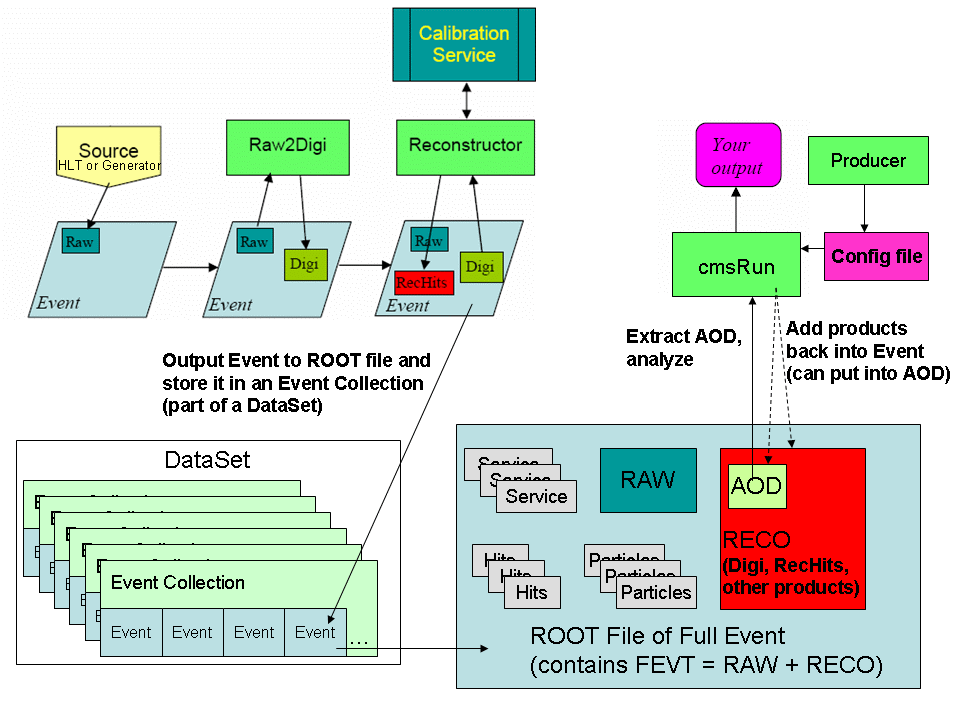
\includegraphics[scale=0.45]{figures/experiment/edm.png} 
\caption{The Event Data Model}
\label{edm}
\end{figure}

An event starts as a collection of the raw data. As the event data is processed, products are stored in the event as reconstructed data objects. The event also contains metadata describing the configuration of the software used for the reconstruction of each object and the conditions for alignment and calibration. %The event data is output to files browsable by ROOT \cite{root}. 
\noindent Analysis Object Data (AOD) is a subset of the reconstructed data sufficient for most analysis to access the relevant objects. 

\subsection{Computing Infrastructure}

CMS makes use of a grid of computers connected together in an hierarchical organisation so that users around the world can share data and computational power. The structure called Worldwide LHC Computing Grid (WLCG) is divided in clusters of computers called Tiers which are classified depending on their computational power and storage capacity.
\begin{compact_itemize}
\item Tier 0: The Tier T0 is located at CERN, where all raw information coming from the detector is saved, reconstructed, and later on transmitted to the rest of the chain. Recently a mirror of the CERN site was deployed at Budapest and they are connected at 100 Gbps to each other;
\item Tier 1: There are fourteen national T1 sites around the world, providing storage and redistribution for MC events generated by the T2's;
\item Tier 2: There T2 centers provides capacity for user analysis, calibration studies, and Monte Carlo production for the whole experiment.   
\item Tier 3: Any small cluster of computers installed at an institute providing local access to the Grid.
\end{compact_itemize}

The S\~ao Paulo Research and Analysis Center (SPRACE) \cite{sprace} was implemented in 2003 to collaborate with the D$\O$ and CMS experiments. SPRACE hosts a T2 of the CMS computing structure --- the BR--SP--SPRACE ---, providing processing power of 25,200 HEPSPEC06 and 1,450 TB of storage, all with a redundant 100 Gbps link to the Fermilab T1 in the USA, which is our main connection to the WLCG. During the development of this work we made extensive use of  the resources of the local CMS center at SPRACE.




